\documentclass[12 pt]{article}         
\usepackage{amsfonts, amssymb}
\usepackage{fancyhdr}
\usepackage{amsmath}
\usepackage{tikz}
\usetikzlibrary{automata, positioning}

\oddsidemargin=-0.5cm                  
\setlength{\textwidth}{6.5in}          
\addtolength{\voffset}{-20pt}        		
\addtolength{\headsep}{25pt}

\setlength{\headheight}{27.2pt}
\addtolength{\topmargin}{-12.7pt}

\pagestyle{fancy}
\fancyhf{}
\fancyhead[L]{Theory and Practice of Algorithms \\ Homework 3}
\fancyhead[R]{Jingheng Huan \\ \today}
\fancyfoot[C]{\thepage}

\begin{document}

\section*{Problem 1}

(a)
\[
\text{L}_1 = (\texttt{+}|\texttt{-})? \left( \texttt{[0-9]*(.)?} \texttt{[0-9]*} \right)
\]

\vspace{20pt}
(b)
\[
L_2 = \left( (a\ |\ b)\ a \right)^*\ (a\ |\ b)?
\]

\vspace{20pt}

\section*{Problem 2}

For the 0*:


\begin{tikzpicture}[shorten >=1pt, node distance=2cm, on grid, auto]
    \node[state, initial, accepting] (q0) {$q_0$};
    \node[state] (q1) [right=of q0] {$q_1$};
    \node[state, accepting] (q2) [right=of q1] {$q_2$};

    \path[->]
    (q0) edge node {$\epsilon$} (q1)
    (q1) edge node {$0$} (q2)
    (q2) edge [bend left] node {$\epsilon$} (q1);

\end{tikzpicture}

\vspace{1cm}

For the 1*:


\begin{tikzpicture}[shorten >=1pt, node distance=2cm, on grid, auto]
    \node[state, initial, accepting] (q0) {$q_0$};
    \node[state] (q1) [right=of q0] {$q_1$};
    \node[state, accepting] (q2) [right=of q1] {$q_2$};

    \path[->]
    (q0) edge node {$\epsilon$} (q1)
    (q1) edge node {$1$} (q2)
    (q2) edge [bend left] node {$\epsilon$} (q1);

\end{tikzpicture}

\vspace{1cm}

For the $0^+$:


\begin{tikzpicture}[shorten >=1pt, node distance=2cm, on grid, auto]
    \node[state, initial] (q0) {$q_0$};
    \node[state] (q1) [right=of q0] {$q_1$};
    \node[state, accepting] (q2) [right=of q1] {$q_2$};
    \node[state] (q3) [right =of q2] {$q_3$};
    \node[state, accepting] (q4) [right =of q3] {$q_4$};

    \path[->]
    (q0) edge node {$0$} (q1)
    (q1) edge node {$\epsilon$} (q2)
    (q2) edge node {$\epsilon$} (q3)
    (q3) edge node {$0$} (q4)
    (q4) edge [bend left] node {$\epsilon$} (q3);

\end{tikzpicture}

For $0^*1^*0^+$:

\begin{tikzpicture}[shorten >=1pt, node distance=1.5cm, on grid, auto]
   \node[state, initial] (q0) {$q_0$};
   \node[state] (q1) [right=of q0] {$q_1$};
   \node[state] (q2) [right=of q1] {$q_2$};
   \node[state] (q3) [below=of q2] {$q_3$};
   \node[state] (q4) [right=of q3] {$q_4$};
   \node[state] (q5) [right=of q4] {$q_5$};
   \node[state] (q6) [below=of q5] {$q_6$};
   \node[state] (q7) [right=of q6] {$q_7$};
   \node[state, accepting] (q8) [right=of q7] {$q_8$};
   \node[state] (q9) [right=of q8] {$q_9$};
   \node[state, accepting] (q10) [right=of q9] {$q_{10}$}; 

   \path[->]
    (q0) edge  node {$\epsilon$} (q1)
    (q0) edge [bend right] node {$\epsilon$} (q3)
    (q1) edge node {$0$} (q2)
    (q2) edge [bend left] node {$\epsilon$} (q1)
    (q2) edge node {$\epsilon$} (q3)
    (q3) edge node {$\epsilon$} (q4)
    (q3) edge [bend right] node {$\epsilon$} (q6)
    (q4) edge node {$1$} (q5)
    (q5) edge [bend left] node {$\epsilon$} (q4)
    (q5) edge node {$\epsilon$} (q6)
    (q6) edge node {$0$} (q7)
    (q7) edge node {$\epsilon$} (q8)
    (q8) edge node {$\epsilon$} (q9)
    (q8) edge node {$\epsilon$} (q9)
    (q9) edge node {$0$} (q10)
    (q10) edge [bend left] node {$\epsilon$} (q9);
\end{tikzpicture}

\section*{Problem 3}

(a)

Let's assume that \( L_1 \) is a regular language. Then, the Pumping Lemma must hold for \( L_1 \).

Let \( n \) be the pumping length given by the Pumping Lemma. We choose the string:
\[
w = 0^n1^{5n + 1}
\]
This string is in \( L_1 \) because:
\[
i = n, \quad j = 5n + 1, \quad \text{and} \quad 5i = 5n < 5n + 1 = j
\]

According to the Pumping Lemma, we can split \( w \) into \( xyz \) such that:
\begin{itemize}
    \item \( |xy| \leq n \)
    \item \( |y| \geq 1 \)
\end{itemize}

Since \( |xy| \leq n \) and \( w \) starts with \( n \) zeros, both \( x \) and \( y \) consist only of zeros. Let:
\[
x = 0^{n - t}, \quad y = 0^t, \quad \text{where} \quad 1 \leq t \leq n
\]
and
\[
z = 1^{5n + 1}
\]
So, \( w = xyz = 0^{n - t} \, 0^t \, 1^{5n + 1} \).


Now, we consider \( k = 2 \) to pump \( y \):
\[
w' = xy^2z = 0^{n - t} (0^t)^2 1^{5n + 1} = 0^{n - t} 0^{2t} 1^{5n + 1} = 0^{n + t}1^{5n + 1}
\]


For \( w' \) to be in \( L_1 \), it must satisfy \( 5i' < j' \), where:
\[
i' = n + t, \quad j' = 5n + 1
\]
\[
5i' = 5(n + t) = 5n + 5t
\]
Now, check if \( 5i' < j' \):
\[
5i' - j' = (5n + 5t) - (5n + 1) = 5t - 1
\]
Since \( t \geq 1 \), we have:
\[
5t - 1 \geq 5(1) - 1 = 4
\]
Therefore:
\[
5i' - j' \geq 4 > 0 \implies 5i' > j'
\]
This means \( 5i' < j' \) is not satisfied, so \( w' \notin L_1 \).

The Pumping Lemma requires that \( xy^kz \in L \) for all \( k \geq 0 \). However, we found \( k = 2 \) such that \( xy^2z \notin L_1 \). This contradiction implies that \( L_1 \) does not satisfy the Pumping Lemma. Since assuming \( L_1 \) is regular leads to a contradiction, we conclude that \( L_1 \) is not a regular language.

\vspace{1cm}

(b)


We are given the language:
\[
L = \left\{ 0^i1^j : i, j \geq 0 \text{ and } (i \bmod 2) + 1 = j \bmod 3 \right\}
\]
with the alphabet \(\Sigma = \{0, 1\}\). We need to write regular expression that represents \(L\).

\subsubsection*{When \(i \bmod 2 = 0\) and \(j \bmod 3 = 1\)}

\begin{itemize}
    \item \(i\) is even: \(i = 2k\) for \(k \geq 0\).
    \item \(j = 1 \mod 3\): \(j = 3m + 1\) for \(m \geq 0\).
\end{itemize}

The regular expressions for these are:

\begin{itemize}
    \item Even number of zeros: \((00)^*\)
    \item Length of ones is equal to \(1 \mod 3\): \((111)^*1\)
\end{itemize}

So, the regular expression for this case is:
\[
R_1 = (00)^*(111)^*1
\]

\subsubsection*{When \(i \bmod 2 = 1\) and \(j \bmod 3 = 2\)}

\begin{itemize}
    \item \(i\) is odd: \(i = 2k + 1\) for \(k \geq 0\).
    \item \(j = 2 \mod 3\): \(j = 3m + 2\) for \(m \geq 0\).
\end{itemize}

The regular expressions for these are:

\begin{itemize}
    \item Odd number of zeros: \((00)^*0\)
    \item Length of ones congruent to \(2 \mod 3\): \((111)^*11\)
\end{itemize}

So, the regular expression for this case is:
\[
R_2 = (00)^*0(111)^*11
\]

The complete regular expression is the union of \(R_1\) and \(R_2\):
\[
R = R_1 \cup R_2 = (00)^*(111)^*1 \cup (00)^*0(111)^*11
\]

\vspace{1cm}

(c)

We are given the language:
\[
L = \left\{ 0^i : \exists k \in \mathbb{N}, \; i = k^2 \right\}
\]
over the alphabet \(\Sigma = \{0\}\). We need to determine whether \(L\) is a regular language. Let's assume that \(L\) is a regular language. Then, it must satisfy the Pumping Lemma.


Let \(n\) be the pumping length given by the Pumping Lemma. We choose the string:
\[
w = 0^{n^2}
\]
This string is in \(L\) because:
\[
i = n^2, \quad \text{and} \quad \exists k = n \text{ such that } i = k^2
\]


According to the Pumping Lemma, we can split \(w\) into \(xyz\) such that:
\begin{itemize}
    \item \( |xy| \leq n \)
    \item \( |y| \geq 1 \)
\end{itemize}

Since \(|xy| \leq n\) and \(w\) consists entirely of zeros, both \(x\) and \(y\) consist of zeros from the first \(n\) symbols of \(w\). Let:
\[
x = 0^{p}, \quad y = 0^{q}, \quad z = 0^{n^2 - p - q}
\]
where \(p \geq 0\), \(q \geq 1\), and \(p + q \leq n\).


When \( k = 2 \):

\[
w' = xy^2z = xyyz = 0^{p}0^{2q}0^{n^2 - p - q} = 0^{n^2 + q}
\]
The length of \(w'\) is:
\[
|w'| = n^2 + q
\]
Since \(q \geq 1\), \( |w'| > n^2 \).

We need to determine whether \( |w'| = n^2 + q \) can still be a perfect square.

For \( w' \) to be in the language \( L \), \( |w'| = n^2 + q \) must also be a perfect square. Let us yze the inequality:
\[
n^2 + q \geq (n + 1)^2
\]
Expanding the right-hand side:
\[
n^2 + q \geq n^2 + 2n + 1
\]
Simplifying this gives:
\[
q \geq 2n + 1
\]

Since \(q\) is a portion of \(y\) with \( |y| \leq n \), it follows that:
\[
q \leq n
\]
However, from the inequality \( q \geq 2n + 1 \), we see a clear contradiction:
\[
n \geq 2n + 1
\]
Simplifying, we get:
\[
n - 2n \geq 1 \implies -n \geq 1,
\]
which is impossible since \( n \geq 1 \).

Therefore, \( |w'| \) is not a perfect square, and \( w' \notin L \). This contradicts the Pumping Lemma, which requires that \( xy^kz \in L \) for all \( k \geq 0 \). The contradiction implies that \( L \) does not satisfy the Pumping Lemma for regular languages. Therefore, \( L \) is not a regular language.

\vspace{1cm}

\noindent\textbf{Collaborators: None}

\end{document}